\chapter{Choix du sujet}

\section{Découverte de Kaggle}
Pour ce projet, je devais choisir moi-même un sujet sur lequel travailler, un domaine ou je devais utiliser des algorithmes d'intelligences artificielles. Je me suis donc rendu sur le site Kaggle qui comprend des compétitions et des datasets. Un dataset est un ensemble de données sur un sujet. Ce site comprend aussi des formations pour prendre en main python et ses bibliothèques pour le traitement des données comme Numpy ou Scikit-Learn. Avant de choisir un dataset pour ce projet, j'ai commencé par effectuer la formation "Python" et "Intro to Machine Learning" qui m'a permis de mieux comprendre l'utilisation de Scikit-Learn.

\section{Pourquoi ce domaine ?}
Une fois une petite base acquise, je me suis rendu sur la catégorie dataset de Kaggle pour voir l'ensemble des datasets disponibles. C'est en faisant mes recherches que j'ai trouvé un dataset contenant des données sur les différents championnats de Formule 1 depuis 1950. La formule 1 est un sport que je suis depuis plus de 10 ans grâce à mon père qui m'a transmis sa passion. Après avoir regardé son contenu et trouver un objectif avec celle-ci, j'ai fait valider mon sujet par Mme. Ansart, ma tutrice du projet, pour pouvoir continuer mon projet avec ce dataset.

\section{Explication de la Formule 1}
Un championnat de Formule 1 est une série de courses automobiles qui se déroule sur un ensemble de courses à travers le monde. Les équipes de F1 sont composées de constructeurs automobiles et de pilotes professionnels qui concourent pour le titre de champion du monde de F1. Les courses se déroulent sur une saison qui dure généralement de mars à décembre, avec des courses chaque week-end. Les pilotes sont classés en fonction de leur performance lors de chaque course, et le pilote ou l'équipe avec le plus de points à la fin de la saison est déclaré champion.\\

Un Grand Prix de Formule 1 est une course qui fait partie de ce championnat. Les Grands-Prix se déroulent sur des circuits de courses spécialement conçus et sont généralement assez longs, avec des longueurs allant de 5 à 7 kilomètres. Avant chaque Grand Prix, il y a des séances d'essais libres et de qualifications pour permettre aux pilotes de se familiariser avec le circuit et de déterminer leur place de départ sur la grille. Les qualifications consistent en plusieurs tours rapides pour déterminer la position de départ des pilotes, avec les meilleurs temps qui obtiennent les positions les plus avancées sur la grille de départ. La course elle-même dure au maximum 2 heures, avec les pilotes qui effectuent un certain nombre de tours du circuit. Les pilotes s'arrêtent pour changer de pneus pendant la course, ce qui peut influencer leur stratégie et leur performance. Seul les dix premiers d'une course gagnent des points allant de 25 à 1 points pour le 10e.


\newpage
\section{Le Dataset}

\href{https://www.kaggle.com/datasets/thedevastator/formula-one-racing-a-comprehensive-data-analysis}{Dataset sur la formule 1 utilisée pour la suite du projet}\\

\subsection{Explication du contenu du dataset}

\subsubsection{Fichier Circuits.csv}
Le fichier Circuits.csv contient l'ensemble des circuits de Formule 1 avec leurs noms, leurs pays et leurs positions géographiques.

\subsubsection{Fichier Constructors.csv}
Le fichier Constructors.csv contient l'ensemble des écuries de Formule 1 qui ont éxisté. Ce fichier liste uniquement les noms des écuries et leurs nationalités. Une écurie de F1 est composé de deux pilotes principaux, de pilote réserviste et de nombreux ingénieurs pour concevoir la voiture et réaliser des stratégies pour les différentes courses.

\subsubsection{Fichier Drivers.csv}
Le fichier Drivers.csv comprend l'ensemble des pilotes qui ont au moins participé à un grand prix de F1. Ce dataset contient aussi le nom, le prénom et la date de naissance de chacun des pilotes.

\subsubsection{Fichier Lap\_times.csv}
Le fichier Lap\_times.csv contient le temps et la position à chaque tours de chaque pilote pour chacun des Grands-prix qu'ils ont effectué. Nous avons à notre disposition le temps en Minute/Seconde/Milliseconde et le temps en Millisecondes ainsi que sa position pour le tour.

\subsubsection{Fichier Pit\_stops.csv}
Le fichier Pit\_stops.csv contient tous les arrêts au stand avec à quel moment de la course un pilote effectue cet arrêt, à quelle tour et la durée de l'arrêt au stand. Durant un Grands-prix, chaque pilote doit au moins effectuer un arrêt au stand pour mettre un autre type de pneus.

\subsubsection{Fichier Qualifying.csv}
Le fichier Qualifying.csv comprend la position du pilote après la séance de classification et ses 3 meilleurs temps des 3 séances de qualifications. Les qualifications se divisent en 3 parties appelées Q1, Q2 et Q3. Après la première séance de qualification Q1, seulement les 15 meilleurs pilotes accèdent à la Q2 et seulement les 10 meilleurs de la séance Q2 accèdent à la dernière séance de qualification Q3 qui déterminera le placement finale sur la grille de départ.

\subsubsection{Fichier Results.csv}
Le fichier Results.csv contient l'ensemble des résultats de chacun des pilotes pour chaque course qu'ils ont effectuée avec leur position, leur nombre de points gagner et leurs positions de départ. C'est un des fichiers les plus importants parce que c'est celui qui contient le nombre de points gagner par course pour chaque pilote et avec son écurie associée.

\subsubsection{Fichier Races.csv}
Le fichier Races.csv contient l'ensemble des grand-prix réalisé depuis 1950 et avec leur date, l'heure et la ville ou se situent le circuit.

\subsubsection{Fichier Constructor\_standings.csv}
Le fichier Constructor\_standings.csv contient le nombre de points et la position au classement de chacune des écuries de Formule 1 pour chaque championnat mondial annuel.

\newpage

A travers l'ensemble de ses fichiers, j'ai sélectionné une partie de ces données qui semblait être le plus intéressant et pertinent pour le sujet choisit qui est : la course, le pilote, l'écurie du pilote, sa position de départ et d'arrivée, son temps de coure en millisecondes, sa position au moment de son meilleur tour ainsi que le numéro du tour en question, sa vitesse moyenne et le nombre de points obtenus. \\

De plus, il nous faut choisir un pilote qui nous servira d'exemple tout long du projet. Pour cela, il faut qu'il est assez d'expérience pour avoir un nombre de données assez importantes qui nous permettrons ensuite effectuer des prédictions. J'ai choisi le  pilote Sebastian VETTEL qui a plus de dix ans d'expérience avec différentes écuries comme Red-Bull où il fut plusieurs fois champion du monde et Ferrari.\\

Nous disposons de 11 colonnes pour 291 lignes d'informations pour le pilote Sebastian VETTEL avec les colonnes citées précédemment.\\

\subsection{Visualisation des données}
\begin{figure}[H]
    \centering
    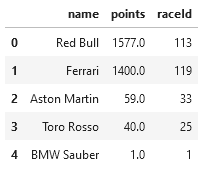
\includegraphics[width=.4\textwidth]{images/VettelEcurieScore.png} 
    \caption{Ensemble des points gagnés et le nombre de course disputée par S. VETTEL pour chacune de ses écuries}
\end{figure}

Ce tableau nous indique que Sebastian VETTEL à disputer un grand nombre de course dans sa carrière et avec des écuries différentes. Cela est intéressant pour les prédictions parce que certaines écuries n'ont pas les mêmes moyens et stratégies ce qui influe sur le résultat final.\\

\begin{figure}[H]
    \centering
    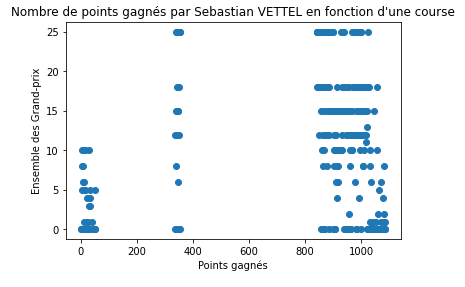
\includegraphics[width=.5\textwidth]{images/VettelRace.png} 
    \caption{Nombre de points gagnés par Sebastian VETTEL en fonction d'une course}
\end{figure}

\begin{figure}[H]
    \centering
    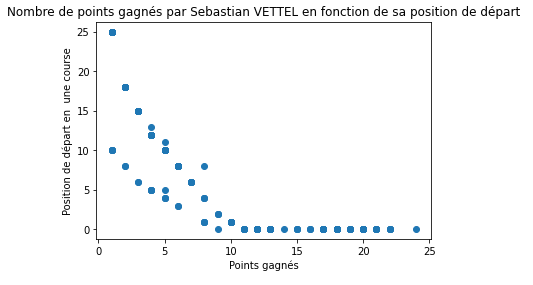
\includegraphics[width=.6\textwidth]{images/VettelPos.png} 
    \caption{Nombre de points gagnés par Sebastian VETTEL en fonction de sa position de départ}
\end{figure}

Ces représentations m'ont permis de prendre en main le Dataset ainsi que de comprendre le jeu de données.





